\documentclass[tikz,border=3pt]{standalone}
\usepackage{amsmath}
\usepackage{tikz}
\usetikzlibrary{shapes.geometric,arrows.meta,patterns,calc}

\begin{document}
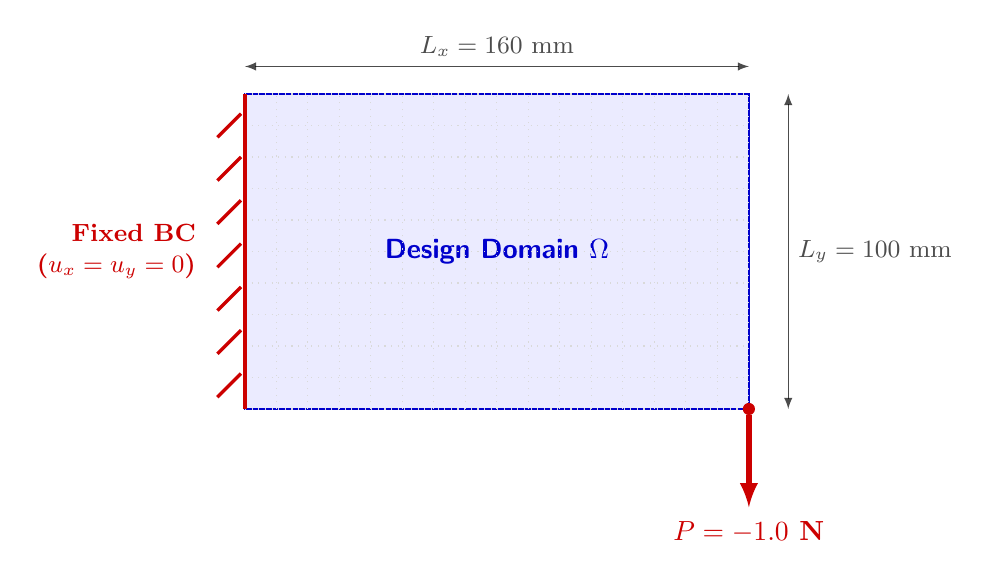
\begin{tikzpicture}[scale=1.0, >=latex]
  % CantileverCorner2d: 160 x 100 mm, 绘图比例 0.04 -> 6.4 x 4.0
  % Design Domain
  \draw[thick, fill=blue!8, draw=blue!80!black] (0,0) rectangle (6.4,4);
  \node[font=\bfseries\sffamily, color=blue!80!black] at (3.2,2) {Design Domain $\Omega$};

  % Grid overlay
  \draw[step=0.4, gray!30, dotted] (0,0) grid (6.4,4);

  % Fully clamped Left Boundary (x=0): u_x = u_y = 0
  \draw[ultra thick, red!80!black] (0,0) -- (0,4);
  \foreach \y in {0.3, 0.85, 1.4, 1.95, 2.5, 3.05, 3.6} {
    \draw[line width=1.2pt, red!80!black] (-0.35, \y-0.15) -- (-0.05, \y+0.15);
  }
  \node[left, red!80!black, font=\small\bfseries, align=right] at (-0.5, 2) {Fixed BC\\($u_x = u_y = 0$)};

  % Concentrated Point Load at Bottom-Right Corner (160, 0)
  \fill[red!80!black] (6.4,0) circle (2.2pt);
  \draw[->, ultra thick, red!80!black, line width=2pt] (6.4, -0.08) -- (6.4, -1.25);
  \node[below, red!80!black, font=\bfseries] at (6.4, -1.3) {$P = -1.0\text{ N}$};

  % Dimensions (顶部与右侧, 避开载荷箭头)
  \draw[<->, opacity=0.7] (0,4.35) -- (6.4,4.35) node[midway, above, font=\small] {$L_x = 160\text{ mm}$};
  \draw[<->, opacity=0.7] (6.9,0) -- (6.9,4) node[midway, right, font=\small] {$L_y = 100\text{ mm}$};
\end{tikzpicture}
\end{document}
